%% NYU PhD thesis format. Created by Jos� Koiller 2007--2008.

%% Use the first of the following lines during production to
%% easily spot "overfull boxes" in the output. Use the second
%% line for the final version.
%\documentclass[12pt,draft,letterpaper]{report}
\documentclass[12pt,letterpaper]{report}

%% Replace the title, name, advisor name, graduation date and dedication below with
%% your own. Graduation months must be January, May or September.
\newcommand{\thesistitle}{Compilation and Tuning of High Level Numerical Programs}
\newcommand{\thesisauthor}{Eric Mann-Hielscher}
\newcommand{\thesisadvisor}{Professor Dennis Shasha}
\newcommand{\graddate}{December 2012}
%% If you do not want a dedication, scroll down and comment out
%% the appropriate lines in this file.
\newcommand{\thesisdedication}{To my dog Weierstra\ss, with affection.}

%% The following makes chapters and sections, but not subsections,
%% appear in the TOC (table of contents). Increase to 2 or 3 to
%% make subsections or subsubsections appear, respectively. It seems
%% to be usual to use the "1" setting, however.
\setcounter{tocdepth}{1}

%% Sectional units up to subsubsections are numbered. To number
%% subsections, but not subsubsections, decrease this counter to 2.
\setcounter{secnumdepth}{3}

%% Page layout (customized to letter paper and NYU requirements):
\setlength{\oddsidemargin}{.6in}
\setlength{\textwidth}{5.8in}
\setlength{\topmargin}{.1in}
\setlength{\headheight}{0in}
\setlength{\headsep}{0in}
\setlength{\textheight}{8.3in}
\setlength{\footskip}{.5in}

%% Use the following commands, if desired, during production.
%% Comment them out for final version.
%\usepackage{layout} % defines the \layout command, see below
%\setlength{\hoffset}{-.75in} % creates a large right margin for notes and \showlabels

%% Controls spacing between lines (\doublespacing, \onehalfspacing, etc.):
\usepackage{setspace}

%% Use the line below for official NYU version, which requires
%% double line spacing. For all other uses, this is unnecessary,
%% so the line can be commented out.
\doublespacing % requires package setspace, invoked above

%% Each of the following lines defines the \com command, which produces
%% a comment (notes for yourself, for instance) in the output file.
%% Example:    \com{this will appear as a comment in the output}
%% Choose (uncomment) only one of the three forms:
%\newcommand{\com}[1]{[/// {#1} ///]}       % between [/// and ///].
\newcommand{\com}[1]{\marginpar{\tiny #1}} % as (tiny) margin notes
%\newcommand{\com}[1]{}                     % suppress all comments.

%% This inputs your auxiliary file with \usepackage's and \newcommand's:
%% It is assumed that that file is called "definitions.tex".
%%
%% Place here your \usepackage's. Some recommended packages are already included.
%%

% Graphics:
\usepackage[final]{graphicx}
%\usepackage{graphicx} % use this line instead of the above to suppress graphics in draft copies
%\usepackage{graphpap} % \defines the \graphpaper command

% Indent first line of each section:
\usepackage{indentfirst}

% Good AMS stuff:
%\usepackage{amsthm} % facilities for theorem-like environments
%\usepackage[tbtags]{amsmath} % a lot of good stuff!

% Fonts and symbols:
%\usepackage{amsfonts}
%\usepackage{amssymb}

\usepackage{listings,fixltx2e,lambda,array,times,color,algpseudocode}
\usepackage{stmaryrd}
\usepackage[usenames,dvipsnames]{xcolor}

\definecolor{lightgray}{rgb}{0.96,0.96,0.96}

\lstset{ 
  language=Python,                % the language of the code
  linewidth=1.0\linewidth, 
  xleftmargin=8pt,
  basicstyle=\footnotesize\ttfamily, % Standardschrift
  numbers=none,                   % where to put the line-numbers
  numberstyle=\footnotesize,          % the size of the fonts that are used for the line-numbers
  stepnumber=1,                   % the step between two line-numbers. If it's 1, each line 
                                  % will be numbered
  numbersep=5pt,                  % how far the line-numbers are from the code
  showspaces=false,               % show spaces adding particular underscores
  showstringspaces=false,         % underline spaces within strings
  showtabs=false,                 % show tabs within strings adding particular underscores
  frame=single,                   % adds a frame around the code
  tabsize=2,                      % sets default tabsize to 2 spaces
  captionpos=b,                   % sets the caption-position to bottom
  breaklines=true,                % sets automatic line breaking
  breakatwhitespace=false,        % sets if automatic breaks should only happen at whitespace
  %title=\lstname,                   % show the filename of files included with \lstinputlisting;
                                  % also try caption instead of title
  numberstyle=\tiny\color{gray},        % line number style
  keywordstyle=\color{blue},          % keyword style
  commentstyle=\color{dkgreen},       % comment style
  backgroundcolor=\color{lightgray}, 
  belowskip=0pt, 
  aboveskip=6pt, 
}

% Formatting tools:
%\usepackage{relsize} % relative font size selection, provides commands \textsmalle, \textlarger
%\usepackage{xspace} % gentle spacing in macros, such as \newcommand{\acims}{\textsc{acim}s\xspace}

% Page formatting utility:
%\usepackage{geometry}

%%
%% Place here your \newcommand's and \renewcommand's. Some examples already included.
%%
% \renewcommand{\le}{\leqslant}
% \renewcommand{\ge}{\geqslant}
% \renewcommand{\emptyset}{\ensuremath{\varnothing}}
% \newcommand{\ds}{\displaystyle}
% \newcommand{\R}{\ensuremath{\mathbb{R}}}
% \newcommand{\Q}{\ensuremath{\mathbb{Q}}}
% \newcommand{\Z}{\ensuremath{\mathbb{Z}}}
% \newcommand{\N}{\ensuremath{\mathbb{N}}}
% \newcommand{\T}{\ensuremath{\mathbb{T}}}
% \newcommand{\eps}{\varepsilon}
% \newcommand{\closure}[1]{\ensuremath{\overline{#1}}}
%\newcommand{\acim}{\textsc{acim}\xspace}
%\newcommand{\acims}{\textsc{acim}s\xspace}

%%
%% Place here your \newtheorem's:
%%

%% Some examples commented out below. Create your own or use these...
%%%%%%%%%\swapnumbers % this makes the numbers appear before the statement name.
%\theoremstyle{plain}
%\newtheorem{thm}{Theorem}[chapter]
%\newtheorem{prop}[thm]{Proposition}
%\newtheorem{lemma}[thm]{Lemma}
%\newtheorem{cor}[thm]{Corollary}

%\theoremstyle{definition}
%\newtheorem{define}{Definition}[chapter]

%\theoremstyle{remark}
%\newtheorem*{rmk*}{Remark}
%\newtheorem*{rmks*}{Remarks}

%% This defines the "proo" environment, which is the same as proof, but
%% with "Proof:" instead of "Proof.". I prefer the former.
%\newenvironment{proo}{\begin{proof}[Proof:]}{\end{proof}}


%% Cross-referencing utilities. Use one or the other--whichever you prefer--
%% but comment out both lines for final version.
%\usepackage{showlabels}
%\usepackage{showkeys}

\begin{document}
%% Produces a test "layout" page, for "debugging" purposes only.
%% Comment out for final version.
%\layout % requires package layout (see above, on this same file)

%%%%%% Title page %%%%%%%%%%%
%% Sets page numbering to "roman style" i, ii, iii, iv, etc:
\pagenumbering{roman}
%
%% No numbering in the title page:
\thispagestyle{empty}
%
\begin{center}
  {\large\textbf{\thesistitle}}
  \vspace{.7in}

  by
  \vspace{.7in}

  \thesisauthor
  \vfill

\begin{doublespace}
  A dissertation submitted in partial fulfillment\\
  of the requirements for the degree of\\
  Doctor of Philosophy\\
  Department of Mathematics\\
  New York University\\
  \graddate
\end{doublespace}
\end{center}
\vfill

\noindent\makebox[\textwidth]{\hfill\makebox[2.5in]{\hrulefill}}\\
\makebox[\textwidth]{\hfill\makebox[2.5in]{\hfill\thesisadvisor\hfill}}
\newpage
%%%%%%%%%%%%% Blank page %%%%%%%%%%%%%%%%%%
\thispagestyle{empty}
\vspace*{0in}
\newpage

%%%%%%%%%%%%%% Dedication %%%%%%%%%%%%%%%%%
%% Comment out the following lines if you do not want to dedicate
%% this to anyone...
%\vspace*{\fill}
%\begin{center}
%  \thesisdedication\addcontentsline{toc}{section}{Dedication}
%\end{center}
%\vfill
%\newpage
%%%%%%%%%%%%%% Acknowledgements %%%%%%%%%%%%
%% Comment out the following lines if you do not want to acknowledge
%% anyone's help...
\section*{Acknowledgements}\addcontentsline{toc}{section}{Acknowledgements}
%% Write your acknowledgements in this file. If you do not want to acknowledge anyone,
%% you can delete this file and comment out the corresponding part in the "thesis.tex"
%% file.
%
I would like to acknowledge the effort put into this thesis by
myself. This work could not have been done without me.

\newpage
%%%% Abstract %%%%%%%%%%%%%%%%%%
\section*{Abstract}\addcontentsline{toc}{section}{Abstract}
%% Write your abstract here.
%
The Riemann Hypothesis has been among the most important open
problems in mathematics for the past 150~years. In this thesis
I solve it, providing a positive result.

\newpage
%%%% Table of Contents %%%%%%%%%%%%
\tableofcontents

%%%%% List of Figures %%%%%%%%%%%%%
%% Comment out the following two lines if your thesis does not
%% contain any figures. The list of figures contains only
%% those figures included withing the "figure" environment.
\listoffigures\addcontentsline{toc}{section}{List of Figures}
\newpage

%%%%% List of Tables %%%%%%%%%%%%%
%% Comment out the following two lines if your thesis does not
%% contain any tables. The list of tables contains only
%% those tables included withing the "table" environment.
\listoftables\addcontentsline{toc}{section}{List of Tables}
\newpage

%%%%% Body of thesis starts %%%%%%%%%%%%
\pagenumbering{arabic} % switches page numbering to arabic: 1, 2, 3, etc.
%% Introduction. If your thesis has no introduction, or chapter 1 is
%% meant to be the introduction, then comment out the lines below.
\section*{Introduction}\addcontentsline{toc}{section}{Introduction}
%% Write your introduction here.
%
This thesis is about the Riemann Hypothesis. We provide an
affirmative answer to the question ``If $z$ is a zero of the
zeta function and $0\le \Re(z)\le1$, then is $\Re(z)$
necessarily equal to $1/2$?''

In chapter~\ref{chap:one} we do this and that.

In the latter chapters we\ldots

%% If your thesis has different "Parts", use commands such as the following:
%\part{First Part\label{part:one}}%
\chapter{The Parakeet Language and Compiler\label{chap:parakeet}}

Parakaeet is awesome and it does cool stuff.


\chapter{Tiling and Unrolling Optimizations\label{chap:optimizations}}

Cache tiling is a classic performance optimization that exploits temporal reuse of data to get maximal benefit from data caches~\cite{Lam91, Wolf91}.  Many numerical computations, including e.g.~dense matrix multiplication, involve significant data reuse due their all-to-all computational pattern.

\begin{lstlisting}[frame=single, label=untiledmm, caption={Untiled Matrix Multiply}, belowskip=0.5em]
for i in range(numRows):
  for j in range(numCols):
    C[i,j] = 0
    for k in range(rowLen):
      C[i,j] += A[i*rowLen + k] * \
                B[j*rowLen + k]
\end{lstlisting}

For example, consider the code for matrix multipication given in Listing \ref{untiledmm}, with a vizualation of the elements accessed to compute a single output value shown in Figure \ref{untiled_diagram}.  If the \lstinline{A} and \lstinline{B} matrices are large, then this code will have poor cache behavior and thus suboptimal performance.  To understand why, consider the data access pattern.  The columns of \lstinline{B} are accessed repeatedly, and thus could benefit from being cached to lower their access times.  However, between each access to an element of \lstinline{B}, the entire rest of \lstinline{B} is accessed, in addition to an entire row of both \lstinline{A} and the output matrix and.  Thus the column of \lstinline{B} will be evicted from the cache between each use, and it will have to be read from a slower level of the memory hierarchy.  Things are similar with the rows of \lstinline{A}.

A better access pattern is one that accesses pieces (called tiles) of the input data at a time such that as much data as possible remains resident in cache between subsequent uses.  Consider the vizualation of a tiled organization of matrix multiply in Figure \ref{tiled_diagram}.  The rows of the \lstinline{A} matrix are grouped into tiles, and each \lstinline{A} tile is entirely consumed before moving onto the next one.  An analagous grouping is done with \lstinline{B}'s columns.  Finally, the iteration through each group of rows and columns is broken up into tiles as well.  Code for this tiling is given in Listing \ref{untiledmm}, where we see that each loop in the original code is broken up into both an outer loop that iterates across tiles and an inner loop that iterates across elements of the current tile.

Consider the data access pattern in this version.  Now rather than the entire matrix \lstinline{B} being accessed between each access to a given element of \lstinline{B}, only an entire \emph{tile} of \lstinline{B} is accessed.  If the tile size is small enough that this tile fits in cache, subsequent accessed to elements of \lstinline{B} will be much faster in this version.  The tile size that works best depends on the size of the cache, the size of the data, and the particular code being executed.

\begin{figure}
\centering
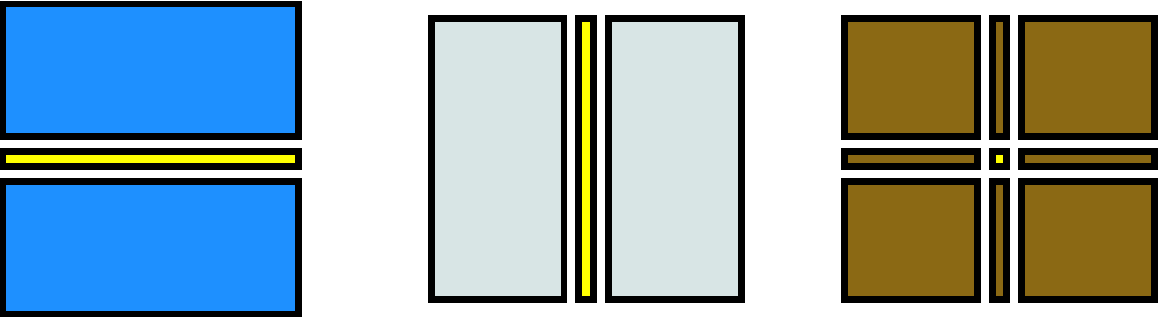
\includegraphics[scale=0.4]{UntiledMMIterationSpace.pdf}
\caption{Untiled Matrix Multiply Iteration Order}
\label{untiled_diagram}
\end{figure}

\begin{figure}
\centering
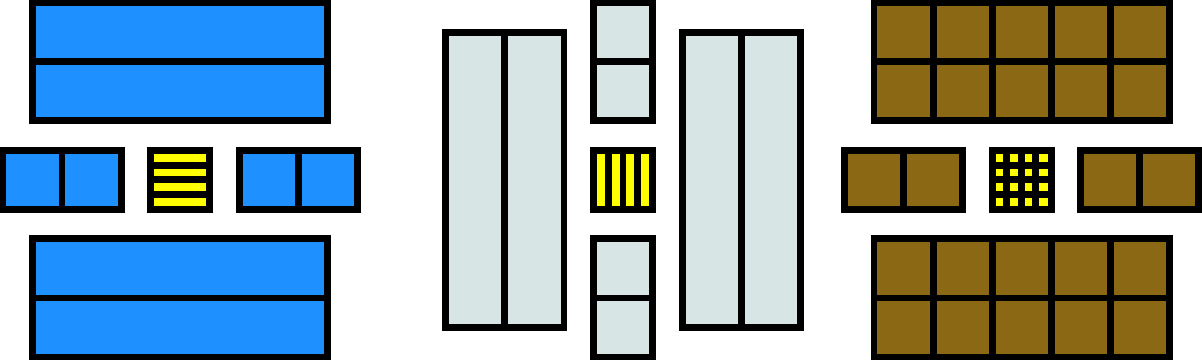
\includegraphics[scale=0.4]{TiledMMIterationSpace.pdf}
\caption{Tiled Matrix Multiply Iteration Order}
\label{tiled_diagram}
\end{figure}

\begin{lstlisting}[frame=single, label=tiledmm, caption={Tiled Matrix Multiply}, belowskip=0.5em]
for at in range(0, numRows, atSize):
  for bt in range(0, numCols, btSize):
    for i in range(at, at+atSize):
      for j in range(bt, bt+btSize):
        C[i,j] = 0
    for kt in range(0, rowLen, ktSize):
      for i in range(at, at+atSize):
        for j in range(bt, bt+btSize):
          for k in range(kt, kt+ktSize):
            C[i,j] += A[rowLen*i + k] * \
                      B[rowLen*j + k]
\end{lstlisting}

Cache tiling need not be for a single level of cache; tiling loops can be added for each level of cache in which to keep data resident between accesses.  In addition, tiling can be used to keep data resident in other levels of the memory hierarchy such as registers.

There has been much work on automating the process of tiling, including both generating the outer tiled loops from the inner ones as well as automating tile size selection given a tiled loop nest~\cite{Lam91, Wolf91} (REFS).  It might appear at first glance that determining good tile sizes for a given loop nest might be easy to do analytically.  Much work has been done on designing analytic models to estimate good tile sizes~\cite{Cole95, Shir12, Yoto03, Yoto05}.  However, while these models often perform fairly well, the state of the art for achieving the best performance is still offline autotuning to find the best settings for a particular target architecture, even for a problem as well-studied as matrix multiplication~\cite{Whal00}.


\chapter{Tiling Adverbs\label{chap:tiling_adverbs}}

\section{Example: Tiling Adverbial Matrix Multiplication\label{sec:adverb_mm}}

In order to understand how our compiler automatically tiles Parakeet code, let us walk through an example.  In Figure \ref{parmm}, we see an implementation of matrix multipication.  This is a desugared version of the actual Parakeet code that we used in our benchmarks in Chapter \ref{chap:evaluation}, altered for ease of presentation to assume that the second input matrix \lstinline{Y} has already been transposed.

\begin{figure}
\begin{singlespace}
\begin{lstlisting}
def dot(x, y):
  return Reduce(lambda x,y,acc: acc + x*y,
                x, y, init=0,
                combiner=lambda x,y: x+y)

def dgemm_1(x, Y):
  return Map(dot, Y, fixed=[x])
                
def dgemm(X, Y):
  return Map(dgemm_1, X, fixed=[Y])
\end{lstlisting}
\end{singlespace}
\label{parmm}
\caption{Parakeet Matrix Multiplication}
\end{figure}

Recall from the discussion in Chapter \ref{chap:optimizations} that the \lstinline{AllPairs} pattern of data access in matrix multiplication involves temporal reuse such that cache tiling is very beneficial for performance.  At a high level, tiling an adverb (or loop) involves wrapping that adverb in another version of itself that breaks up its iteration pattern into smaller pieces.  The outer adverb iterates over tiles, while the inner one performs the original computation on the individual elements of each tile.

To support tiling in our compiler we introduce a set of \emph{tiled adverbs}, one for each existing adverb.  At a high level, the semantics of a tiled adverb are that it splits its inputs along some axis into tiles.  These tiles are then each consumed by executing the tiled adverb's nested function, and these partial results are combined in some structured way to form the final result.  Definitions of tiled adverbs' semantics are given in Figure \ref{def_tiled_adverbs}.  Note that our actual implementations of tiled adverbs are more efficient than these definitions might suggest.  The \lstinline{Split} operator in Figure \ref{def_tiled_adverbs} splits its arguments into tiles along the specified axis.  However, the actual tile sizes are left unspecified -- in the case of cache tiling until runtime, and in the case of register tiling until final compile time.

To see the problem with this, let's examine its cache behavior in detail.  Assume that we're tiling for L1 cache and that the matrices are much larger than the size of L1 cache so that even a single row from either matrix is on the order of the size of the cache (a realistic assumption for even medium sized data and current cache sizes).

First, the rows of the matrices \lstinline{X} and \lstinline{Y} are split into tiles.  Then, for every pair of tiles, every pair of rows from the tiles is passed to the function \lstinline{tiled_dot}.  At this point we can see that the \lstinline{TiledAllPairs} isn't going to do much to help cache behavior, as the single rows of the matrices are already large compared with the cache and so grouping them into even larger tiles is useless.

The next step of the computation involves splitting each pair of rows from \lstinline{X} and \lstinline{Y} into tiles, and then performing a dot product between each of these pieces.  Finally, these partial dot products are combined via addition to produce a final result.  In contrast with the \lstinline{TiledAllPairs}, the tiles from the \lstinline{TiledReduce} are able to benefit cache behavior, as they can be made small enough to fit into cache.  However, since they are splitting single rows of \lstinline{X} and \lstinline{Y}, the tiles' shapes are forced to be 1xN for some N.  It has been shown in various studies of tiling that the best tile shapes are typically closer to square, and ATLAS only considers square tiles in its search (REFS).  Regardless, we want the runtime's search to be able to find the best tile shapes and thus prefer not to restrict their shape in any way.

Thus we see that this straightforward approach to tiling the adverbs is problematic.  What we'd really prefer is for all of the tiling of every adverb to happen first, and then once the inputs are broken up into cache-friendly pieces only then to perform the inner computation.  A tiled version of matrix multiply that adheres to this principle is shown in Listing \ref{good_tiled_adverb_mm}.

\begin{figure}
\begin{singlespace}
\begin{lstlisting}
def dot(x, y):
  return Reduce(lambda x,y,acc: acc + x*y,
                x, y, init=0,
                combiner=lambda x,y: x+y)

def dgemm(X, Y):
  return AllPairs(dot, X, Y)

def tiled_dot(X, Y):
  return TiledReduce(dgemm, X, Y,
                     init=0, axes=[1,1],
                     combiner=lambda x,y: x+y)

def tiled_dgemm_1(x, Y):
  return TiledMap(tiled_dot, Y, fixed=[x])
                     
def tiled_dgemm(X, Y):
  return TiledMap(tiled_dgemm_1, X, fixed=[Y])
\end{lstlisting}
\end{singlespace}
\label{good_tiled_adverb_mm}
\caption{Good Tiled Matrix Multiplication}
\end{figure}

The difference between this code and the last is that it's organized in the way we want: all of the tiling happens first, and the inner computation is performed on the cache-friendly pieces of the inputs. This solves both problems with the first version: the tiling of the \lstinline{TiledAllPairs} is now relevant in fitting the inner computation into cache, and all axes of the cache-relevant tiles' shapes are now free parameters that are settable at runtime.

\section{Adverb Tiling Algorithm\label{sec:adverb_tiling_algorithm}}

While the transformation ``nest all tilings, then all original computation'' is legal in the case of matrix multiply, the case of general code is more complicated.  This is due to various factors such as the presence of additional non-adverb statements in functions which are tiled and control flow.  The full algorithm for our tiling transformation is given if Figure \ref{tiling_algorithm}.

\begin{figure*}
\centering
\begin{tabular}{| m{0.01cm}llm{10.8cm} |}
\hline
& & &\\
& function   & $::=$ & $\lambda x_1,\ldots,x_n.$statement$^+$\\
& statement  & $::=$ & $x$ \textbf{= } expression $|$ \textbf{return} expression\\
& expression & $::=$ & \textbf{map}($f$, $e_1,\ldots,e_n$) $|$ \textbf{reduce}($f$, $combiner, e_{init}, e_1,\ldots,e_n$)\\
&            &       & $|$ $e_1 \oplus e_2 $ $|$ $e_1[e_2]$ $|$ $x$\\
& & &\\
\hline
\end{tabular}
\caption{Simplified Parakeet Syntax}
\label{tiling_syntax}
\end{figure*}

\begin{figure*}
\centering
\begin{tabular}{| m{0.01cm}llm{9.5cm} |}
\hline
& & &\\
& $\llbracket\textbf{\textrm{return}}$ $e\rrbracket^{\alpha,\epsilon}_{stmt}$ & $::=$ & \textbf{return} $\llbracket e \rrbracket^{\alpha,\epsilon}_{expr}$\\
& & &\\
\hline
\end{tabular}
\caption{Adverb Tiling Transformation Algorithm}
\label{tiling_algorithm}
\end{figure*}

Before tiling an AST, we normalize every compound expression by breaking it up into a series of statements each of which only contains simple expressions.

\section{Comparison with the Polyhedral Model\label{sec:polyhedral_comparison}}

The Polyhedral Model is a well-studied method for modeling the iteration spaces and data dependencies of statements in loop nests.  The high level model represents these as a series of matrices which enables performing various loop optimizations including tiling, skewing, and automatic parallelization via algebraic transformations of these matrices~\cite{Bena10,Bond08,Hart09,Pouc10,Wolf91a,Wolf91b}.


\chapter{Experimental Evaluation\label{chap:evaluation}}

In this chapter, evaluate our compiler's performance via a series of experiments.

\section{Tiling Performance}

Here we'll show tiling performance.  Yep.


%%%%% Appendices start %%%%%%%%%%%%%%%%
%% Comment out the following line if your thesis has no appendix
%\appendix
%\input{app1}
%% Note: If your thesis has more than one appendix, NYU requires a "list of
%% appendices" page before the body of the thesis. I don't provide the tools
%% to create that here, so you're on your own for that one... Sorry.
%\input{app2}
%%%% Input bibliography file %%%%%%%%%%%%%%%

\bibliographystyle{abbrv}
\bibliography{../Parakeet}{}

\end{document}
